% !TEX root = ../documento.tex
%% ========================================================================== %%
%% Capítulo 3 - Análise do Sistema (versão revisada para comparação)         %%
%% ========================================================================== %%

\chapter{Análise do Sistema} \label{cap:analise-revisado}

Este capítulo transforma a compreensão do contexto operacional do Apache Gru Rock Bar e das necessidades identificadas em uma visão estruturada do sistema \textbf{Karaokê Apache}. O objetivo é definir o que o sistema deve fazer, quem interage com ele, quais conceitos compõem seu domínio, quais requisitos devem ser atendidos e quais restrições condicionam seu desenvolvimento e sua operação.

A análise mantém o foco no comportamento esperado do sistema e nas regras do negócio. As decisões relacionadas à arquitetura, às tecnologias, à organização dos componentes e aos detalhes de implementação são apresentadas nos capítulos posteriores.

\section{Visão Geral do Sistema}

O sistema \textbf{Karaokê Apache} foi concebido como uma plataforma distribuída centrada na orquestração da fila de reprodução musical. Sua finalidade é substituir o fluxo manual de pedidos por um processo organizado, no qual o cliente solicita uma música, acompanha a fila e aguarda sua vez, enquanto o organizador administra as apresentações e controla a reprodução da música ativa no telão.

O sistema possui três áreas funcionais principais:

\begin{itemize}
  \item \textbf{Solicitação de músicas:} permite que o cliente se identifique, pesquise uma música disponível e solicite sua inclusão na fila;
  \item \textbf{Administração da fila:} permite que o organizador acompanhe, ordene, inicie, avance ou remova pedidos;
  \item \textbf{Exibição da apresentação:} atualiza instantaneamente o estado da música ativa para que o reprodutor desktop dedicado renderize o vídeo correspondente em tela cheia na TV do bar.
\end{itemize}

O limite do sistema começa no acesso do cliente à interface de solicitação e termina na atualização do estado do pedido e na exibição da música ativa. O sistema não substitui a atuação do organizador, o equipamento de áudio ou a operação artística do evento. Também não é responsável pela produção do conteúdo audiovisual nem pela disponibilidade dos vídeos de terceiros.

\section{Atores Envolvidos}

Foram identificados três atores que interagem diretamente com o sistema ou com seus resultados. Os gestores do estabelecimento são partes interessadas do projeto, mas não constituem um ator operacional separado quando utilizam as mesmas funcionalidades do administrador.

\begin{table}[H]
\IBGEtab{%
  \caption{Atores envolvidos no sistema Karaokê Apache.}%
  \label{tab:atores-revisado}%
}{%
  \footnotesize
  \begin{tabularx}{\textwidth}{p{3.5cm}p{2.8cm}X}
    \toprule
    \textbf{Ator} & \textbf{Tipo} & \textbf{Papel no sistema} \\
    \midrule
    \textbf{Cliente (Cantor)} & Humano, primário & Identifica-se no sistema, pesquisa uma música, solicita sua inclusão na fila e acompanha a posição do pedido e a música em execução. \\
    \addlinespace
    \textbf{Administrador (Organizador)} & Humano, primário & Controla a operação do karaokê, inicia apresentações, avança a fila, remove pedidos e acompanha o estado geral do evento. \\
    \addlinespace
    \textbf{Reprodutor de Telão} & Sistema externo, secundário & Recebe a indicação da música ativa e apresenta o conteúdo audiovisual no telão. \\
    \bottomrule
  \end{tabularx}%
}{%
  \fonte{Elaborado pelos autores (2026).}
}
\end{table}

\section{Casos de Uso}

Os casos de uso descrevem as funcionalidades sob a perspectiva dos atores e representam os comportamentos relevantes para a operação do sistema. O diagrama da Figura \ref{fig:casos_uso-revisado} apresenta a relação entre os atores e os casos de uso principais.

\begin{figure}[H]
  \caption{Diagrama de Casos de Uso UML do sistema Karaokê Apache.}
  \label{fig:casos_uso-revisado}
  \begin{center}
    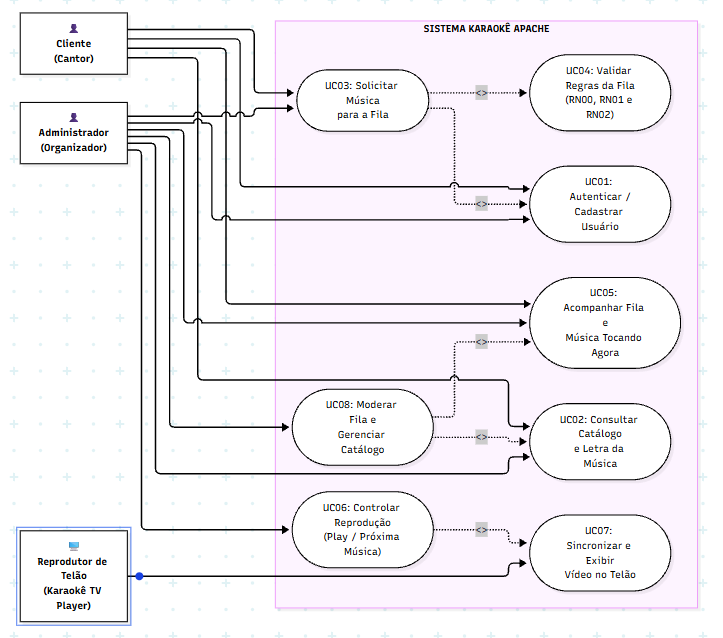
\includegraphics[width=0.92\textwidth]{imagens/DiagramaCasoDeUso.png}
  \end{center}
  \legend{Fonte: Elaborado pelos autores (2026).}
\end{figure}

Os casos de uso foram organizados conforme a necessidade que atendem. O caso de uso UC04 é incluído por UC03, pois suas validações fazem parte da solicitação de uma música. O caso de uso UC07 representa a comunicação do estado da fila com o reprodutor de telão, sem definir a tecnologia utilizada para essa comunicação.

\begin{table}[H]
\IBGEtab{%
  \caption{Visão geral dos casos de uso do sistema Karaokê Apache.}%
  \label{tab:casos_uso-revisado}%
}{%
  \footnotesize
  \begin{tabularx}{\textwidth}{p{1.2cm}p{3.2cm}p{2.5cm}X}
    \toprule
    \textbf{Código} & \textbf{Caso de uso} & \textbf{Atores} & \textbf{Objetivo e fluxo principal} \\
    \midrule
    UC01 & Identificar participante & Cliente, Administrador & O ator informa os dados necessários para acessar as funcionalidades correspondentes ao seu perfil. O sistema valida a identificação e apresenta a área autorizada. \\
    \addlinespace
    UC02 & Pesquisar e escolher música & Cliente, Administrador & O ator informa título ou artista, consulta os resultados disponíveis e seleciona uma música para continuar a solicitação. \\
    \addlinespace
    UC03 & Solicitar música para a fila & Cliente & O cliente confirma a música escolhida. O sistema executa UC04 e, se as regras forem atendidas, registra o pedido no final da fila. \\
    \addlinespace
    UC04 & Validar solicitação de música & Sistema, incluído em UC03 & O sistema verifica a disponibilidade da música, a existência de duplicidade e o limite de pedidos ativos do participante. Em caso de falha, rejeita a solicitação e informa o motivo. \\
    \addlinespace
    UC05 & Acompanhar fila e música atual & Cliente, Administrador & O ator visualiza a música em execução, os próximos pedidos e a posição dos itens na fila. \\
    \addlinespace
    UC06 & Controlar apresentação & Administrador & O organizador inicia um pedido, encerra a apresentação atual ou avança para o próximo item, atualizando o estado da fila. \\
    \addlinespace
    UC07 & Atualizar exibição do telão & Reprodutor de Telão & O sistema informa a música ativa e o reprodutor apresenta o conteúdo correspondente. Quando não há música ativa, o telão exibe o estado de espera. \\
    \addlinespace
    UC08 & Moderar fila & Administrador & O organizador remove um pedido, limpa a fila ao encerrar o evento ou corrige uma situação excepcional conforme as regras do estabelecimento. \\
    \bottomrule
  \end{tabularx}%
}{%
  \fonte{Elaborado pelos autores (2026).}
}
\end{table}

\section{Modelo Conceitual}

O modelo conceitual representa os principais conceitos do domínio e os relacionamentos entre eles, sem definir tecnologias, componentes ou operações de implementação. A Figura \ref{fig:classes_conceitual-revisado} apresenta a representação conceitual do sistema.

\begin{figure}[H]
  \caption{Diagrama de Classes Conceitual UML do sistema Karaokê Apache.}
  \label{fig:classes_conceitual-revisado}
  \begin{center}
    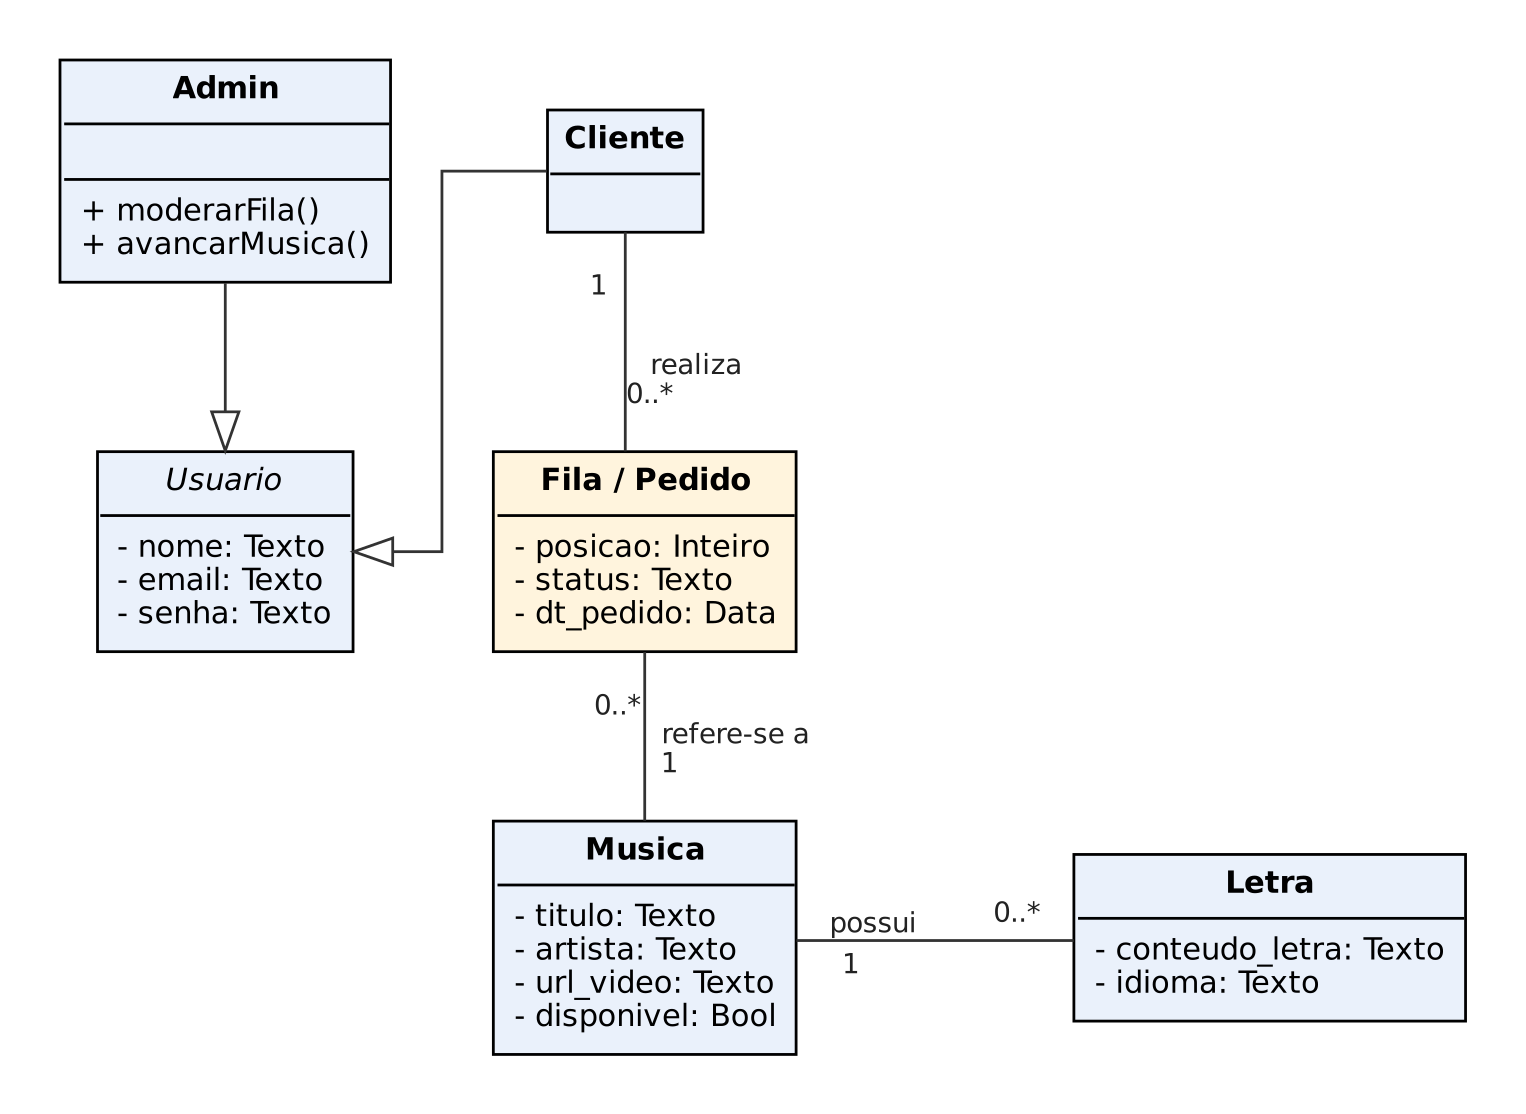
\includegraphics[width=\textwidth,height=0.78\textheight,keepaspectratio]{imagens/diagrama_classes_conceitual.png}
  \end{center}
  \legend{Fonte: Elaborado pelos autores (2026).}
\end{figure}

Os conceitos principais são:

\begin{itemize}
  \item \textbf{Usuário:} representa uma pessoa identificada no sistema. Seus papéis podem ser especializados em \textbf{Cliente} e \textbf{Administrador}, conforme as permissões necessárias para a operação;
  \item \textbf{Cliente:} representa o participante que solicita músicas e acompanha a fila;
  \item \textbf{Administrador:} representa o organizador responsável pelo controle das apresentações;
  \item \textbf{Música:} representa uma opção musical disponível para solicitação, com título, artista e referência ao conteúdo audiovisual;
  \item \textbf{Pedido:} representa a solicitação de uma música feita por um cliente, contendo posição, data da solicitação e estado do atendimento;
  \item \textbf{Letra:} representa o conteúdo textual associado a uma música. No escopo atual, é um conceito previsto para evolução futura e não constitui funcionalidade essencial do MVP.
\end{itemize}

As relações fundamentais do domínio são: um cliente pode realizar vários pedidos; cada pedido é realizado por um único cliente; cada pedido refere-se a uma música; uma música pode ser referenciada por vários pedidos ao longo de diferentes sessões; e cada pedido possui um estado pertencente ao ciclo de atendimento definido pelas regras de negócio.

\section{Requisitos Funcionais}

Os requisitos funcionais especificam os serviços e comportamentos que o sistema deverá oferecer para atender às necessidades N01 a N04 identificadas no contexto do projeto.

\begin{table}[H]
\IBGEtab{%
  \caption{Requisitos funcionais do sistema Karaokê Apache.}%
  \label{tab:requisitos_funcionais-revisado}%
}{%
  \footnotesize
  \begin{tabularx}{\textwidth}{p{1.3cm}p{3.4cm}X p{1.8cm}}
    \toprule
    \textbf{Código} & \textbf{Requisito} & \textbf{Descrição} & \textbf{Prioridade} \\
    \midrule
    RF01 & Identificação de usuário & Permitir que o participante ou organizador se identifique e receba acesso às funcionalidades correspondentes ao seu papel. & Média \\
    \addlinespace
    RF02 & Pesquisa de músicas & Permitir a pesquisa de músicas por título ou artista. & Alta \\
    \addlinespace
    RF03 & Seleção de música & Permitir que o usuário selecione uma música entre os resultados disponíveis. & Alta \\
    \addlinespace
    RF04 & Inclusão de pedido & Permitir que o cliente confirme uma música e inclua o pedido no final da fila. & Alta \\
    \addlinespace
    RF05 & Validação do pedido & Validar disponibilidade, duplicidade e limite de pedidos antes da inclusão na fila. & Alta \\
    \addlinespace
    RF06 & Acompanhamento da fila & Exibir a música ativa, os próximos pedidos e a posição dos itens na fila. & Alta \\
    \addlinespace
    RF07 & Início de apresentação & Permitir que o administrador inicie a apresentação de um pedido selecionado. & Alta \\
    \addlinespace
    RF08 & Avanço da fila & Permitir que o administrador encerre a apresentação atual e avance para o próximo pedido. & Alta \\
    \addlinespace
    RF09 & Moderação de pedidos & Permitir que o administrador remova pedidos individuais ou limpe a fila ao final do evento. & Alta \\
    \addlinespace
    RF10 & Exibição da música ativa & Apresentar no telão a música atualmente em execução e um estado de espera quando não houver apresentação. & Alta \\
    \addlinespace
    RF11 & Atualização do estado do pedido & Registrar as transições entre os estados \textit{Na Fila}, \textit{Reproduzindo}, \textit{Concluído} e \textit{Cancelado}. & Alta \\
    \addlinespace
    RF12 & Feedback das operações & Informar o resultado das ações realizadas, incluindo confirmações, falhas de validação e indisponibilidade de conexão. & Alta \\
    \bottomrule
  \end{tabularx}%
}{%
  \fonte{Elaborado pelos autores (2026).}
}
\end{table}

\subsection{Critérios de aceitação dos requisitos centrais}

Os requisitos centrais devem ser verificáveis por meio de cenários de uso. A Tabela \ref{tab:criterios_aceitacao-revisado} apresenta critérios de aceitação iniciais para o MVP.

\begin{table}[H]
\IBGEtab{%
  \caption{Critérios de aceitação dos requisitos centrais.}%
  \label{tab:criterios_aceitacao-revisado}%
}{%
  \footnotesize
  \begin{tabularx}{\textwidth}{p{1.5cm}X}
    \toprule
    \textbf{Req.} & \textbf{Critério de aceitação} \\
    \midrule
    RF04/RF05 & Dado que a música esteja disponível e não esteja duplicada, ao confirmar a solicitação o sistema deverá criar um pedido na última posição da fila. \\
    \addlinespace
    RF05 & Dado que a música já esteja na fila ou em reprodução, ao tentar solicitá-la novamente o sistema deverá rejeitar o pedido e informar o motivo. \\
    \addlinespace
    RF06 & Dado que existam pedidos ativos, ao acessar a fila o usuário deverá visualizar a música atual e a ordem dos próximos pedidos. \\
    \addlinespace
    RF07/RF08 & Dado que o administrador inicie ou avance uma apresentação, o estado do pedido deverá ser atualizado e o próximo item deverá assumir a condição correspondente. \\
    \addlinespace
    RF10 & Dado que exista uma música ativa, o reprodutor deverá apresentar o conteúdo correspondente no telão; sem música ativa, deverá apresentar o estado de espera. \\
    \addlinespace
    RF12 & Dado que uma operação seja rejeitada ou concluída, o sistema deverá apresentar uma mensagem que permita ao usuário compreender o resultado. \\
    \bottomrule
  \end{tabularx}%
}{%
  \fonte{Elaborado pelos autores (2026).}
}
\end{table}

\section{Requisitos Não Funcionais}

Os requisitos não funcionais definem características de qualidade e condições de operação que complementam os requisitos funcionais. Eles devem ser validados posteriormente por testes, inspeções ou análise da documentação técnica.

\begin{table}[H]
\IBGEtab{%
  \caption{Requisitos não funcionais do sistema Karaokê Apache.}%
  \label{tab:requisitos_nao_funcionais-revisado}%
}{%
  \footnotesize
  \begin{tabularx}{\textwidth}{p{1.4cm}p{2.6cm}p{3.4cm}X}
    \toprule
    \textbf{Código} & \textbf{Categoria} & \textbf{Requisito} & \textbf{Critério esperado} \\
    \midrule
    RNF01 & Usabilidade & Acesso simples em dispositivos móveis & O cliente deverá conseguir acessar a solicitação sem instalar um aplicativo adicional e concluir o fluxo com poucas etapas. \\
    \addlinespace
    RNF02 & Usabilidade & Legibilidade em ambiente noturno & As informações essenciais deverão apresentar contraste e tamanho adequados para o uso em um bar com pouca iluminação. \\
    \addlinespace
    RNF03 & Desempenho & Atualização da fila & Uma alteração de estado deverá ser refletida nos participantes e no telão em tempo compatível com a operação do evento, com meta de até dois segundos na rede local. \\
    \addlinespace
    RNF04 & Compatibilidade & Acesso por navegadores comuns & A interface do cliente deverá funcionar nas versões atuais dos principais navegadores para dispositivos móveis. \\
    \addlinespace
    RNF05 & Segurança & Controle de acesso & Apenas o administrador poderá executar ações de controle da fila e da apresentação. \\
    \addlinespace
    RNF06 & Segurança e privacidade & Proteção dos dados pessoais & A coleta deverá limitar-se aos dados necessários para identificar o participante e operar a fila. \\
    \addlinespace
    RNF07 & Confiabilidade & Consistência dos estados & O sistema não deverá permitir transições incompatíveis ou perda da ordem dos pedidos durante uma operação normal. \\
    \addlinespace
    RNF08 & Manutenibilidade & Separação de responsabilidades & A solução deverá manter separadas as responsabilidades de identificação, pedidos, fila, reprodução e administração. \\
    \bottomrule
  \end{tabularx}%
}{%
  \fonte{Elaborado pelos autores (2026).}
}
\end{table}

\section{Restrições do Sistema}

O desenvolvimento e a operação do sistema estão sujeitos às seguintes restrições:

\begin{itemize}
  \item \textbf{Dependência de conectividade:} os participantes e o equipamento de exibição dependem de conexão adequada durante o evento para consultar a fila, atualizar estados e acessar o conteúdo audiovisual;
  \item \textbf{Disponibilidade de conteúdo de terceiros:} determinados conteúdos podem não permitir reprodução no ambiente utilizado, o que pode impedir ou interromper a apresentação de uma música;
  \item \textbf{Infraestrutura existente:} a solução deve operar com os equipamentos disponíveis no estabelecimento, incluindo dispositivos móveis dos clientes, computador de controle, telão e sistema de som;
  \item \textbf{Restrição orçamentária:} o projeto deve evitar custos de licenciamento incompatíveis com a realidade do estabelecimento parceiro;
  \item \textbf{Proteção de dados pessoais:} a coleta, o armazenamento e o uso de dados dos participantes devem observar os princípios da Lei Geral de Proteção de Dados Pessoais (LGPD), especialmente necessidade, finalidade e transparência \cite{brasil2018lgpd};
  \item \textbf{Regras operacionais do evento:} a ordem dos pedidos, o limite de solicitações por participante e as ações de moderação devem respeitar as políticas definidas pelo organizador karaokê.
\end{itemize}

\subsection{Rastreabilidade entre necessidades, regras e requisitos}

A Tabela \ref{tab:rastreabilidade-revisado} relaciona as necessidades identificadas no contexto às regras de negócio, aos casos de uso e aos requisitos funcionais correspondentes.

\begin{table}[H]
\IBGEtab{%
  \caption{Matriz de rastreabilidade da análise do sistema.}%
  \label{tab:rastreabilidade-revisado}%
}{%
  \footnotesize
  \begin{tabularx}{\textwidth}{p{1.2cm}p{3.0cm}p{2.0cm}p{2.0cm}X}
    \toprule
    \textbf{Nec.} & \textbf{Necessidade} & \textbf{Regras} & \textbf{Casos de uso} & \textbf{Requisitos funcionais} \\
    \midrule
    N01 & Escolha de música pelo próprio sistema & RN00 & UC01, UC02, UC03, UC04 & RF01 a RF05 \\
    \addlinespace
    N02 & Transparência da fila & RN04 & UC05, UC07 & RF06, RF10, RF11, RF12 \\
    \addlinespace
    N03 & Prevenção de repetições e rotatividade & RN01, RN02 & UC03, UC04, UC06, UC08 & RF04, RF05, RF07 a RF09, RF11 \\
    \addlinespace
    N04 & Automação da reprodução no telão & RN03, RN04 & UC06, UC07, UC08 & RF07 a RF12 \\
    \bottomrule
  \end{tabularx}%
}{%
  \fonte{Elaborado pelos autores (2026).}
}
\end{table}

%% -------------------------------------------------------------------------- %%
